\documentclass[conference]{IEEEtran}



\usepackage{graphicx}
\usepackage{subfigure}
\usepackage{graphicx}
\usepackage{caption}

\usepackage[utf8]{inputenc} % Kullanılan encodinge göre utf8 yerine latin5 de yazılabilir.
\usepackage[T1]{fontenc}

\hyphenation{op-tical net-works semi-conduc-tor}


\begin{document}

\title{Distributed Online Training Simulation for Railway Dispatcher }



\author{\IEEEauthorblockN{Nuri Ozalp, Ahmet Basgoze, Ozdemir Kavak, Burcu Kalkan}
\IEEEauthorblockA{TUBITAK BILGEM BTE\\Informatics and Information Security Research Center\\ Information Technologies Institute\\
Kocaeli, Turkey 41470\\
Email: {(nuri.ozalp, ahmet.basgoze, ozdemir.kavak, burcu.kalkan)}@tubitak.gov.tr}
}

\maketitle

\begin{abstract}
Computerized simulations might be thought of as powerful tools to learn analyses, design and interaction. Train traffic simulations are important tools at a critical level. The basic aim of train control systems is preventing trains from collision with other trains, and keeping them at a safe distance.
The main aim of this study is providing train traffic control training for dispatchers in a distributed simulation system. There are instructor console, 5 student consoles, a scenario-editor console and traingraph tools in the system. The system uses actual train routes of Turkey (3 train lines, 50 stations and interlocking areas). In this simulation system, the dispatcher may control the train   traffic at various complexity levels. The success levels of the trainees can be measured in this system. The instructor console makes decisions on the organization of the training and learning experiences, classroom management, and responses to individual   students during the simulation. The user is enabled to follow and track the progress of 5 students during the simulation

\end{abstract}

\section{INTRODUCTION}
Train has an important place in land and railway transportation and consists of train coaches pushed and pulled by one or several locomotives used for transportation. It is an already known fact that trains have an important place in travel and transportation of goods and humans. Various traffic control systems have been developed all over the world due to the increasing railway traffic. The train traffic management methods have various train traffic control system in the world. 
The systems used for railway traffic management are central systems, and are operated by dispatches. The purpose of the dispatches is making the trains reach their targets safely and timely. 
Train traffic control systems are very critical systems. The instant real-time position is not known in conventional trains. With the help of the signalization systems, the nearly-exact positions of the trains are estimated with a 3-km error rate. For this reason, train traffic becomes more critical. Training the dispatchers has become more important with the increasing train routes and increasing number of the train travels in recent years. Training dispatchers by making them work in real train traffic to acquire experience takes long time and brings several risks together with it. For this reason, training simulation systems are needed, and there are many training simulations developed on this topic. Especially, it is necessary that more than one dispatch work together in control centers, and therefore 
there is the need for multiple-user simulation systems with distributed-structure have gained importance. With the help of these systems, it is important that more than one dispatches work together in one single simulation with intense traffic scenario managing the traffic and coping with various problems. 
In this study, the aim is training the dispatches by using the simulation system infrastructure, making them become ready for real train traffic and become specialists in a relatively short time period. A railway system is formed in the simulation where there are intense traffic and various types of trains. The, problems like switches, signals, rails, grade-crossing failure and similar possible problems are created in this simulation system and all these processes are recorded as a scenario. The recorded scenarios are opened in a simulation by the instructor and 5 students may be trained simultaneously. The performances of the students are assessed by observing their processes and reactions and they are given certificates. 
The simulation system has been developed, modeled and introduced to the system in agreement with the actual railway systems for Turkey with 3 different real railway lines. One of these is a fast train line, the second one is a suburban line, and the last one is a conventional train line. The students are trained in the current system in these 3 different railway lines by using characteristic differences for students. 
The simulation system consists of 5 modules, which are;
\begin{itemize}
\item The Trainer Console,
\item The Trainee Console,
\item The Scenario Editor,
\item The Performance Assessment Module,
\item The Train Graf Module. 
\end{itemize}

Apart from these, some other helpful devices have also been developed in this area. The Track-Designer is the most important of these. With this device, the interlocking fields to be modeled are drawn in visual style, and modeled in accordance with the actual models. With Track-Designer, the destinations on one route have been found, the physical characteristics in the field are modeled (determining the positions of signal, switch and similar field equipment), and the production of interlocking tables have been realized. Nearly all of the data needed by the system have been produced by using the Track-Designer. 
 
With the scenario editor, the desired field is prepared, and trains may be added to different positions in the number as many as the editor wishes, and the desired conditions may be created in the field. The conditions that may be created in the field include a possible crash, region time permission, derailment, violation of the red signal, red cross, locomotive breakdown, train/coach escape, signal breakdown, switch breakdown, violation of the speed limit, grade crossing failure. By using the created scenario, the trainers may start one single simulation or 5 different simulations simultaneously, and make any necessary interventions during the simulations. If the trainer wishes, s/he may repeat a scenario with snapshots is it is important for several times. The students may manage trains in the field that are given authorities, and try to solve the problems when they occur. Instant movements of the trains in the simulation may also be monitored with the traingraph. At the end of the training, the trainer may conduct examinations to measure the performances of the students and assess the dispatches with pointing system as Successful/Failed. 
In the 2nd Part, the information on the related work is given. In the 3rd part, information on the infrastructure of the communication system is given. In the 4th Part, the five modules of the system are introduced. The experiments on the system and their results are given in the 5th Part. The conclusion part is in the 6th Part.

\section{RELATED WORK}


The simulations with distributed structures in which more than one dispatches are trained are used commonly. Similar studies are explained in this part. 
Middelkoop et al. conducted a study and used a Simulator called Flexible Rail Infra Simulation of Operations (FRISO). It has an automatic simulation model and is connected to a database. It also has an editing and generator functions, and enables the user to perform single and multiple simulation experiments (stochastic). FRISO also has track layout, signaling system, route setting, and interlocking functions. On the other hand, our system has multiple screen option, and enables 5 students to use the system simultaneously \cite{FRISO}.

 Baohua et al. conducted a study about multiple-training simulator. The simulator can assess the performances on the railway lines, signal layout optimization, energy-efficient operating strategies, exploring the bottleneck problems in traffic, assessment of the reliability of the timetables that are scheduled, and the train delay propagation. The above-mentioned are performed automatically in the multiple-train simulator; however, they are performed by dispatches in our system \cite{ICVES}.

Dispatchers in railways, perform the process of traffic control. In this research about the railway traffic control and train scheduling problem . An algorithm proposed which is different from those of the existing ones. This algorithm is constructed on inter-train conflict resolution and for an alternative solution it reaches a decision by using a look-ahead method. The purpose of this algorithm is to prevent train conflict.
Collision is a major problem but it is only one of those which can be confronted. Dispatcher can learn how to act by our system when they come across to detailed problems like switch failure or isgnal failure \cite{Sahin}.



\section{SYSTEM DESIGN}
\subsection{Simulation Life Cycle}

The RAYTES system is capable of running five independent simulation media simultaneously and independently from each other. In Figure  Şekil \ref{fig:simyasamdongusu} below, the lifecycle represents a simulation medium. When the system is first operated,  
it is in IDLE mode. When a scenario is loaded to the system and a simulation medium is created, it switched to LOADED mode. In this situation, the simulation is at the standby mode and is ready for operation. When the simulation is operated, it switched to RUNNING mode. In RUNNING mode, the simulation time progresses, the objects simulated flow in a time-sensitive manner, and an interaction between the human interfaces and the system is realized. The simulation may be paused at any time. In such a situation, the simulation is in PAUSE mode. The simulation time and simulation processes are paused temporarily in PAUSE mode.  The RUNNING mode can be started again in the PAUSE mode. When the simulation is terminated, the system switched to TERMINATED mode, and cannot be started again. 




\begin{figure}[h!]
  \centering
  % Requires \usepackage{graphicx}
  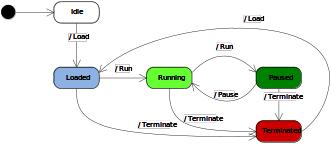
\includegraphics[width=8cm]{simyasamdongusu.jpg}
  \caption{Representation of Simulation Life cycle}\label{fig:simyasamdongusu}
\end{figure}

\subsection{Comminication}
\subsubsection{ Simulation Message}
Simulation Message is the message type of the system in command and control center. These messages are produced in the trainer console, and sent to the other components of the system. It includes the creation, pausing, receiving a snapshot and similar commands of the simulation. In addition, several special intervention commands are defined for the purpose of intervention to the status of the virtual field objects in the simulation.  
\subsubsection{Request Message}
This message type has the commands that are sent to the Control Center Server (CCS) by the Control Center Client (CCC) module. It is the “Client-Server” architecture between the CCC and CCS. The Request Message commands are assessed by the client as the request for service by the client.

\subsubsection{State Message}

hese messages are used for the purpose of sending the status information of the defined elements in the virtual field during the simulation study. The Control Center Server module (CCS) sends the field information to the Control Center Client module (CCC) by using State Message. The Control Center Server module also sends information to the Wide Screen Console (WSC) and to the Trainer Field Intervention (TFI) modules that need to monitor the field via State Message.

\subsubsection{System Message}
These messages are used between the Student Control Management (SCM) and CCS modules. 
This message type is used to ensure that the students who want to be included in the training system to login to the system.
\subsection{Modbus}
Modbus automation is a raw data communication protocol which is accepted in industrial areas. This protocol works with “client-server” logic and used in questioning and transferring the bit series among the systems. In RAYTES Project, modbus packages are transferred to the other modules from the software module over the UDP/IP. The data and command transfer among modules is performed via CCS Module, interlocking Simulator (AS) module, Field Simulator (FS) module and Train Simulator (TS) modules. 


\subsection{SSY Simulation Server Manager Module}
SSM, i.e. the Simulation Server Management Module is the module in which all the active modules in the simulation system are depending in terms of communication infrastructure and coordination. In Figure \ref{fig:syySequenceDiagram}, the Sequence Diagram is given; and in Figure \ref{fig:syygrafic}, the Interface is given. 
All the active modules that are responsible for a duty in simulation flow have to be connected to this module either directly or indirectly over the main module under which that operates \cite{network1,network2,network3,network4}. All the messaging that occurs during the simulation work and its preparation are performed over this module. SSM can also share the data in itself with the other consoles or applications that correspond to relevant messages. SSM uses the Simulation Support (SS) and Messaging Module for messaging like the other system units. This unit receives all the entry data over the SS, and distributes the output data to the system over SS. SS is used in a style that is defined with Message Server duty on SSM. Each message coming to SSM is processed with a pre-control process, and the system decides what to do with the message. There are 4 processes that may be performed on a message by the SSM;

\begin{itemize}
\item Sending the message directly to the target or targets
\item Broadcasting the message to the whole network
\item If the content of the message is related with SSM, sending an answer message to SSM, 
\item If the message must be sent hierarchically, ensuring this hierarchy.  
\end{itemize}






\begin{figure}[h!]
  \centering
  % Requires \usepackage{graphicx}
  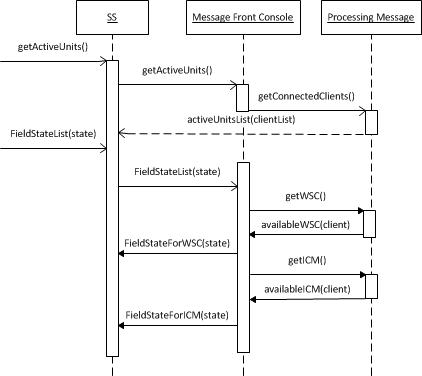
\includegraphics[width=8cm]{syySequenceDiagram.jpg}
  \caption{Representation of SYY squence diagram}\label{fig:syySequenceDiagram}
\end{figure}


\begin{figure}[h!]
  \centering
  % Requires \usepackage{graphicx}
  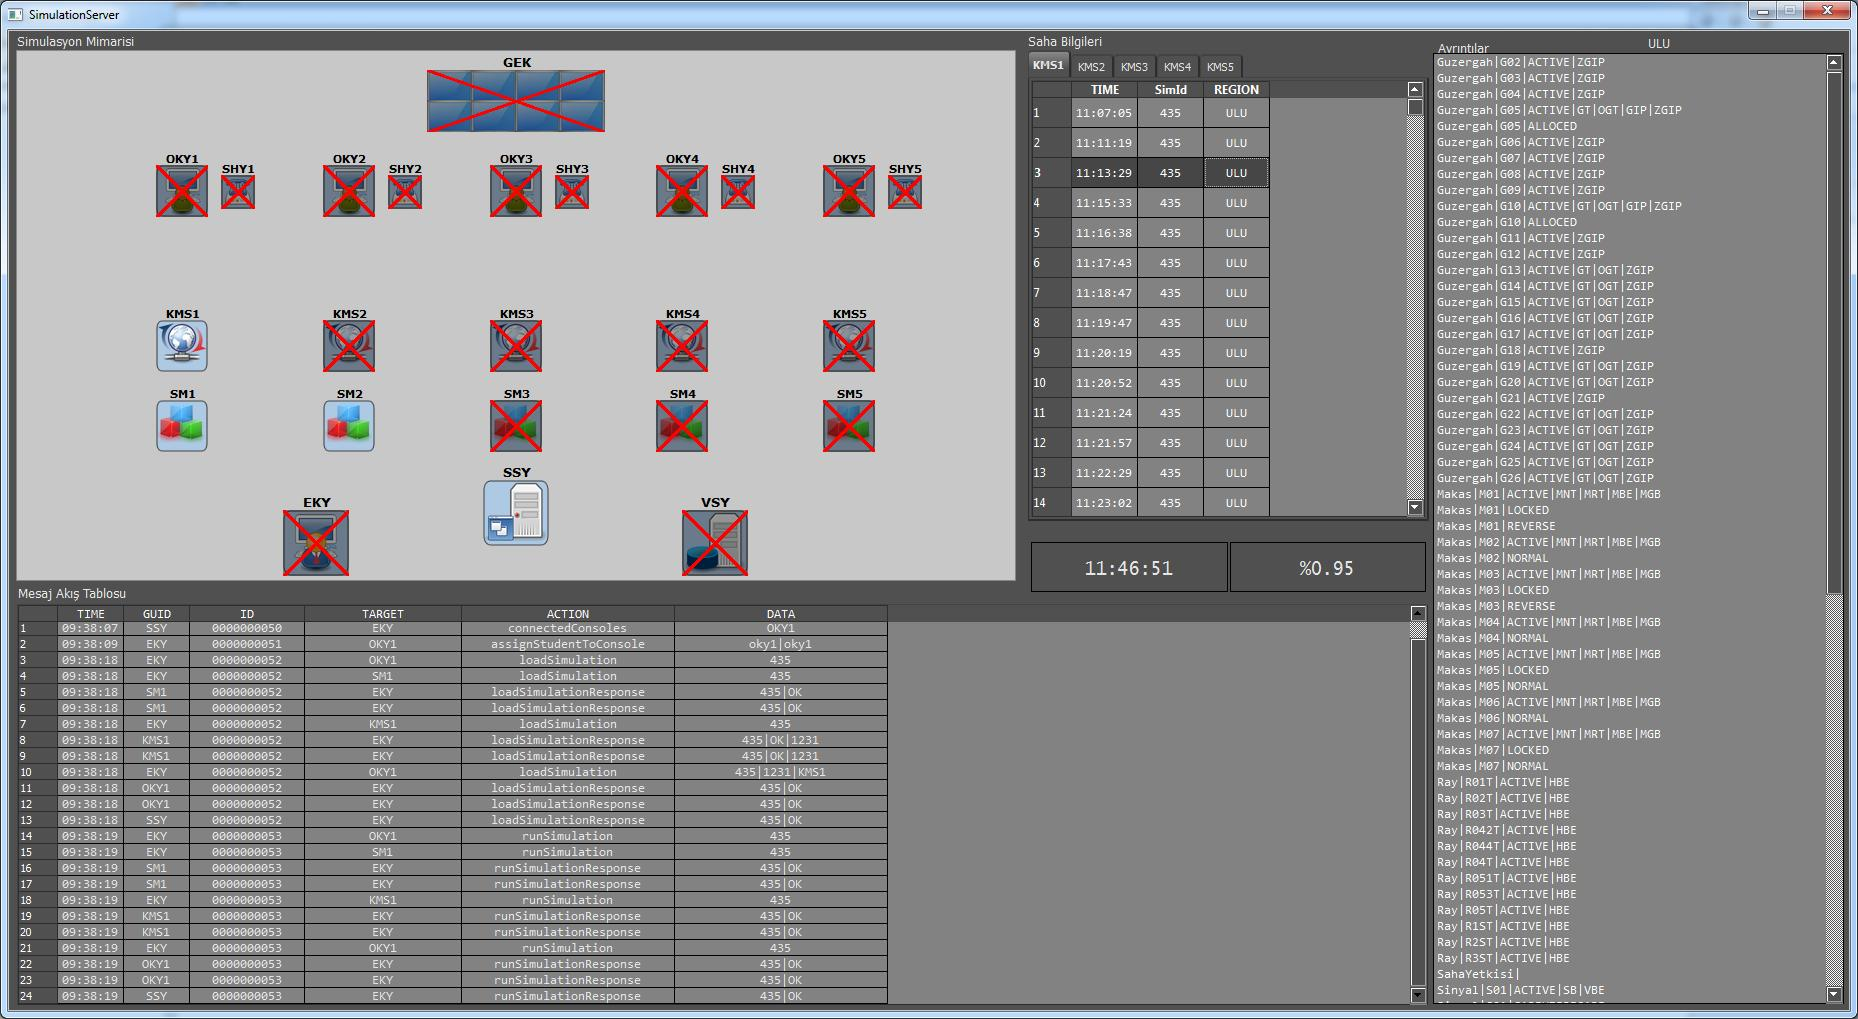
\includegraphics[width=8cm]{syygrafic.jpg}
  \caption{Representation of SYY UI}\label{fig:syygrafic}
\end{figure}

Sending a message hierarchically means sending a message for example a simulation loading message to each unit in priority order. Each message that is sent hierarchically is a positive answer comes; it is transferred to the other relevant unit. If this chain is broken in some point, the system returns the negative message to the first unit that sent the message. If the message cycle is completed, a positive message is transferred \cite{network2}. 

\subsection{Simulation Motor (SM) Module}
\subsubsection{Class Structure: Simulation Motor (SM)}
The main class shown in Figure \ref{fig:smgrafic} is the SimMotor. This class creates and uses the Config, XmlUtility, FieldEventList, FTSimManager::FTSimMgr and Communicator::Client.

FTSimMgr is defined in Field Traffic Simulation Management (FTS) Module. The SimMotor has access to the interlocking, field and traffic simulation modules over the interface provided by FTSimMgr class. The Client Class, which is defined in Communicator Module, provides messaging interface to the SimMotor class. SimMotorGui provides graphic window interface for the purpose of debug and test.


\begin{figure}[h!]
  \centering
  % Requires \usepackage{graphicx}
  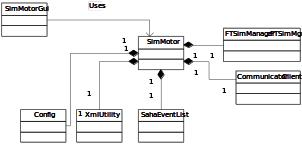
\includegraphics[width=8cm]{smgrafic.jpg}
  \caption{Representation of SM class diagram}\label{fig:smgrafic}
\end{figure}



\subsubsection{Messaging}

When the SSM starts initially, it creates 5 independent SM processes. With the help of these SM processes, 5 independent simulations are controlled by the SSM simultaneously. SSM Simulation Message transfers these types of messages to SM. These messages are upper-level control messages like load simulation, start simulation. SM transfers these messages to Field Traffic Management (FTM) simulation modules. When the simulation module completes the processes that are required by these messages, it sends a reply (positive or negative) to the SM, and this result is informed (feedback) to the SSM. If the LoadSimulation message is taken as a general example, when this message is received by SM, two processes are triggered. The first one is the pre-programs events that have to be played in the scenario are read from the database, and loaded to the Field Event List (FEL) list. Each of these events is defined as Field Event (FE). The second process is the loading of FTS and the Field Simulation Model in it, Interlocking Simulation model and Traffic Simulation model and the technical parameters of the relevant scenario from the database, and preparation of the simulation for start. When the Simulation is running, the FE events which are in the order in the FEL are transferred to FTS modul to be processed according to the simulation time. This mechanism ensures that a scenario is operated without interventions. However, it is also possible to intervene to the simulation by the trainer. The trainer may use the Trainer Field Intervention (TFI) tool and create a manual Field Event. When these FE that are created manually are transferred to the SM instantly, FE adds the event to the top of the FEL list, and ensures that the simulation activates it in the next operation. This work flow is shown in the diagram in Figure  \ref{fig:smCommunicationDiagram}.

\begin{figure}[h!]
  \centering
  % Requires \usepackage{graphicx}
  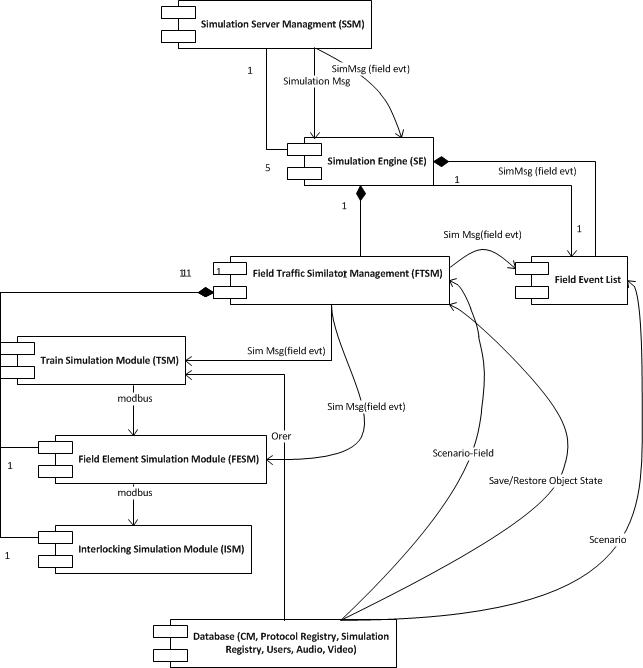
\includegraphics[width=8cm]{smCommunicationDiagram.jpg}
  \caption{Representation of SM Comminication diagram}\label{fig:smCommunicationDiagram}
\end{figure}

\subsubsection{Simulation Support and Messaging Module}

As observed in Figure \ref{fig:RepresentationSDDiagram}, Simulation Support and
Messaging Module are physically independent in the project; however, the units that are in
communication and interaction with each other  communicate together. The communication module, which is established on basic server client architecture, is added disconnection control, single connection property, XML-based message control properties, which are specific to the project, and designed in the light of the protocol rules that are specific to the project. The main module that provides messaging and communication is enabled to work in two modes. The first one is the Server Mode, and the other one is Client mode. When it works in Server mode, the communicating is ensured over a certain connection port. In the second mode, it awaits for the other system to be connected to it.


\begin{figure}[h!]
  \centering
  % Requires \usepackage{graphicx}
  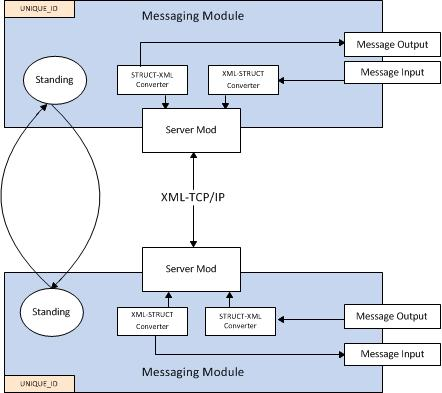
\includegraphics[width=8cm]{RepresentationSDDiagram.jpg}
  \caption{Representation of SD  diagram}\label{fig:RepresentationSDDiagram}
\end{figure}

The client mode will ensure access with a target server data and introduce itself with a unique ID during connection. IP numbers will not be used to make this connection unique.
Because different applications must have the ability to communicate with each other via the same device. When more than one access trials are made with the same ID, the system
will reject the 2nd connection trial with a warning “ID on Use”. As observed in Figure 7, all the clients connected to a server sends the information to the sever that they are “awake” periodically. When considered in reverse angle, the server works with all clients connected to it; in other words, the information that they are “awake” is sent periodically. With this system, the connection control of all the units in the
system is enabled.


\begin{figure}[h!]
  \centering
  % Requires \usepackage{graphicx}
  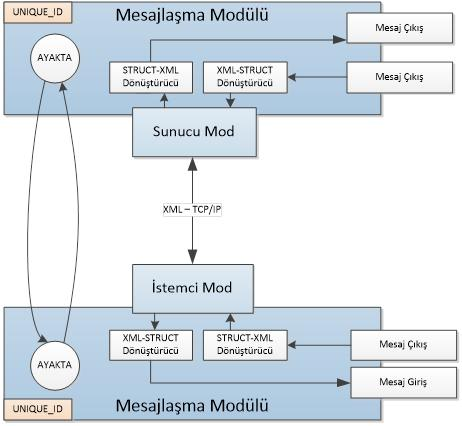
\includegraphics[width=8cm]{SDDiagram.jpg}
  \caption{Representation of SD  diagram}\label{fig:SDDiagram}
\end{figure}



\section{Training Environment}

\subsection{StudentConsole (SC)}

StudentConsole (SC) consists of a Student  Computer Unit(SCU)   and   the   sub-hardware   components   of   a   VoiceCommunication Device (VCD) The structure of SC is shownin  Figure??.  Student  Console  Management  is  an  upper-levelmodule,  and  is  responsible for  the general  functioning of theconsole. The dispatch interface application is performed by theCCC,   and   the   video   recordings   are  performed   by  VideoRecording Infrastructure Module.

\begin{figure}[h!]
  \centering
  % Requires \usepackage{graphicx}
  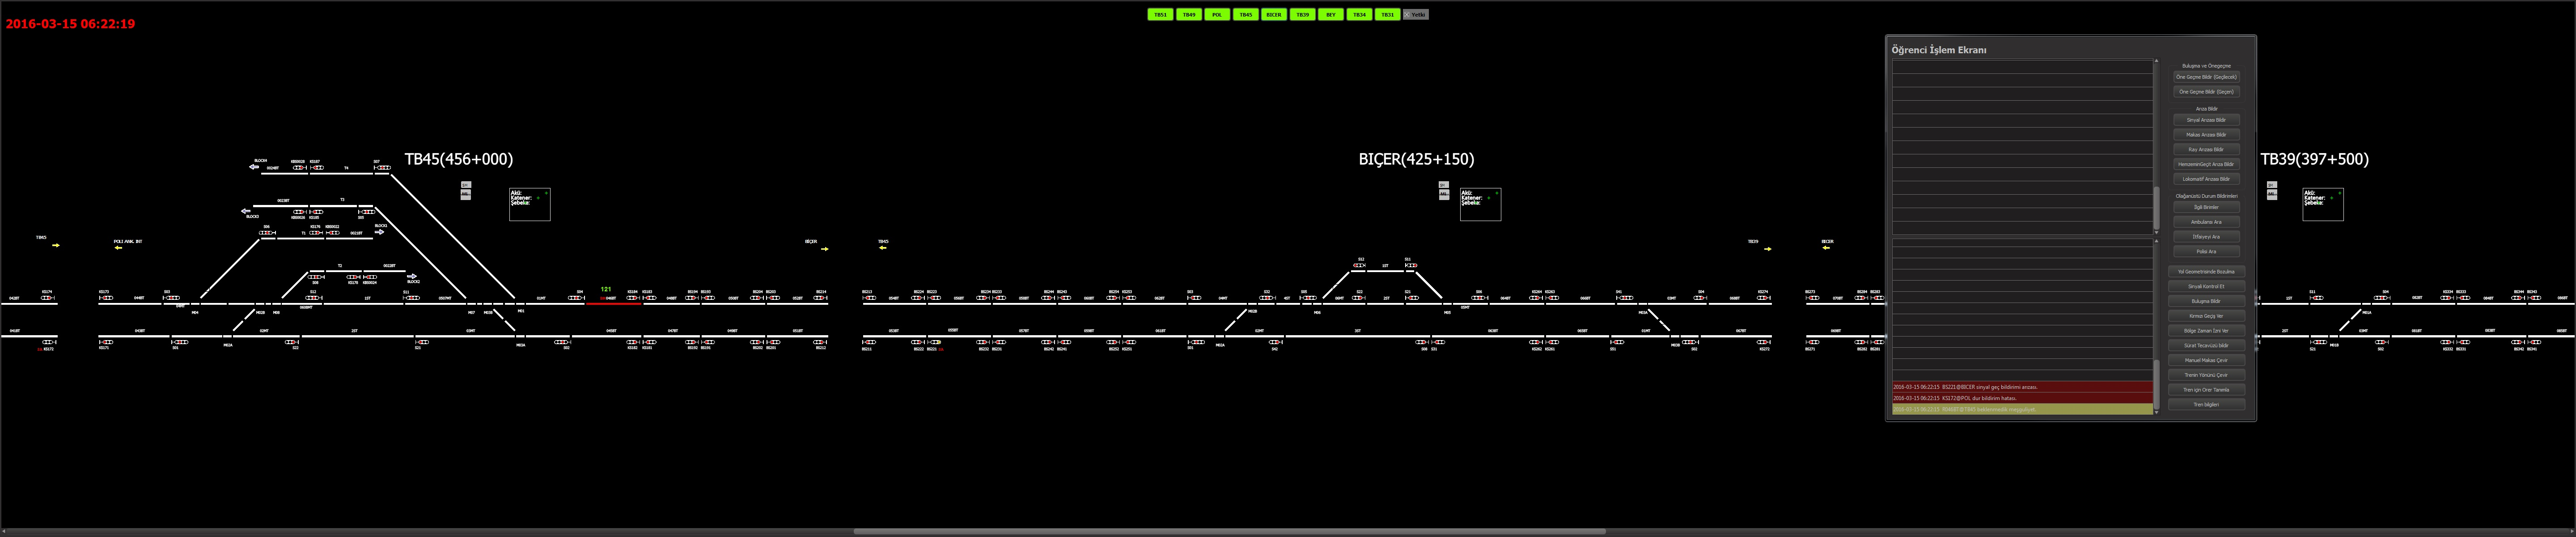
\includegraphics[width=8cm,height=5cm]{ogrenci.jpg}
  \caption{Representation of Dispatcher Console}\label{fig:smclass}
\end{figure}



\subsection{Wide Screen Console (WSC)}

Wide   Screen   Console (WSC) consists of a Wide ScreenComputer Unit (WCU) and a multiple-output displa ycard, and each output is connected to one screen of the WideScreen  Wall  Unit.WCU is designed as a wall with 8 LCDscreens in two lines and four columns.


Wide Screen Management (WSM) software is responsible forthe  running  and  control of CCC,  which are the dispatchinterface application, Video Recording Infrastructure  (VRI)and Video Playback Device (VPD) modules.

In Figure \ref{fig:genisekranSonuc}, the result of an experiment of a wide screen is given.

\subsection{Trainer Console}

The Trainer Console (TC) is the one that can start a simulation and assign students and scenarios to the console. It may intervene to the simulation during the operation. It may
pause, continue or terminate the simulation. It may approve the demands of the students, and take Snapshots. The feedbacks of the students during an examination and grade them. In Figure \ref{fig:egitmenSonuc}, the screenshot of an experiment with trainer module is given.



\subsection{Simulation Server Unit (SSU)}

The Simulation Server Unit (SSU) is used for the purpose of ensuring the coordination between the messaging in RAYTES Project. The duties of it are synchronizing and coordinating the basic functions and the simulation components developed by the project team, displaying all the message flows, the working of the system, awakening the components that constitute the simulation infrastructure, keeping the connection data of the components, and sharing them with other components.
All the active components of the simulation system will be connected either directly or indirectly to the simulation server.
\subsection{Editor Analysis Console}

Scenario Editor Tool (SET), Performance Analysis Tool (PAT), User Management Tool (UMT), Student Education Register Tool (SERT) and Video Playback Tool (VPT) software modules work on Editor Analysis Console (EAC). The preparation of the scenarios before the simulation, defining the users, analyzing the performances after simulation and examining the student training registers is possible with EAC. Therefore, this console is intended for “off-line” use not to be used during the simulation. 

\subsection{Train Graph}
The Traingraph component, which is developed in the scope of the Raytes Project, is a data analysis tool which enables the questioning of train movement (TrainEvent) graphics and shown on graphics with various choices. With the questioning, the movements of the trains on the blocks is monitored. 
A sample view has been provided in Figure \ref{fig:trenGrapSonuc}.


\begin{itemize}
\item The points marked on the left of the curve show the entry of the train to the blocks,
\item The points marked on the right of thecurve show the exit of the train from theblocks,
\item İThe transparent part between the lines show the difference between the entry and exit, i.e. it shows how long the train stayed in this block.
\end{itemize}

Which of these choices are to be shown may be chosen bythe use.In Figure \ref{fig:trenGrapSonuc}, the screenshot of thetraingraph is given.
\section{EXPERIMENT RESULT}
In  the  RAYTES  Project  with  its  distributed  structure,  weperformed the testing of the simulation in 2 different formsfor 5 students who can be trained simultaneously.The first one was planned as a 1-hour scenario in which therewere 5 trains for 5  users who were authorized.   At the end ofthe training, the total RAM and CPU use is given in Figure 9 \ref{fig:hepsibir}.


\begin{figure}[h!]
  \centering
  % Requires \usepackage{graphicx}
  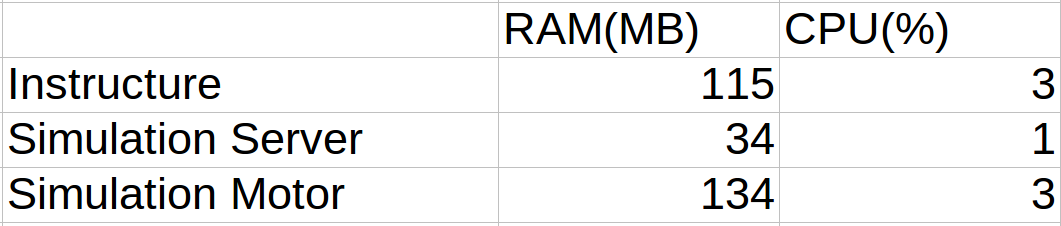
\includegraphics[width=8cm]{hepsibir.png}
  \caption{The  source use of the modules in one single simulation for 5 different  students.}\label{fig:hepsibir}
  
\end{figure}

The second test was planned in the same scenario for 1 hour and in 5 different simulation sessions as 1 student in 1 simulation. At the end of the training, the total RAM and CPU uses are given in Figure \ref{fig:hepsiayri}.

\begin{figure}[h!]
  \centering
  % Requires \usepackage{graphicx}
  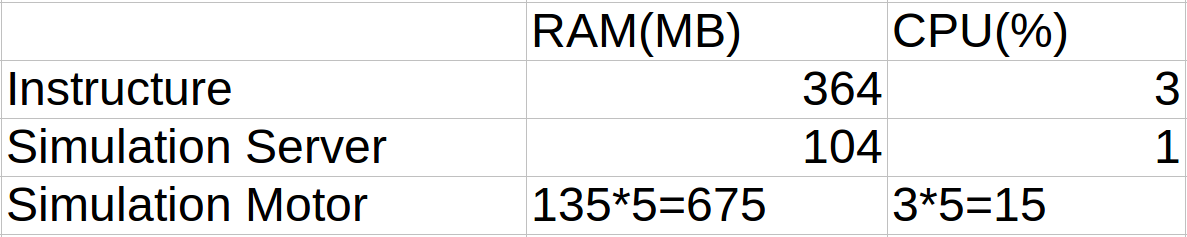
\includegraphics[width=8cm]{hepsiayri.png}
  \caption{The source use of the modules in 5 simulations for 5 different students.}\label{fig:hepsiayri}
  
\end{figure}

The traingraph showing the movements of the trains at the end of the experiment is given in the Figure \ref{fig:trenGrapSonuc}. 
\begin{figure}[h!]
  \centering
  % Requires \usepackage{graphicx}
  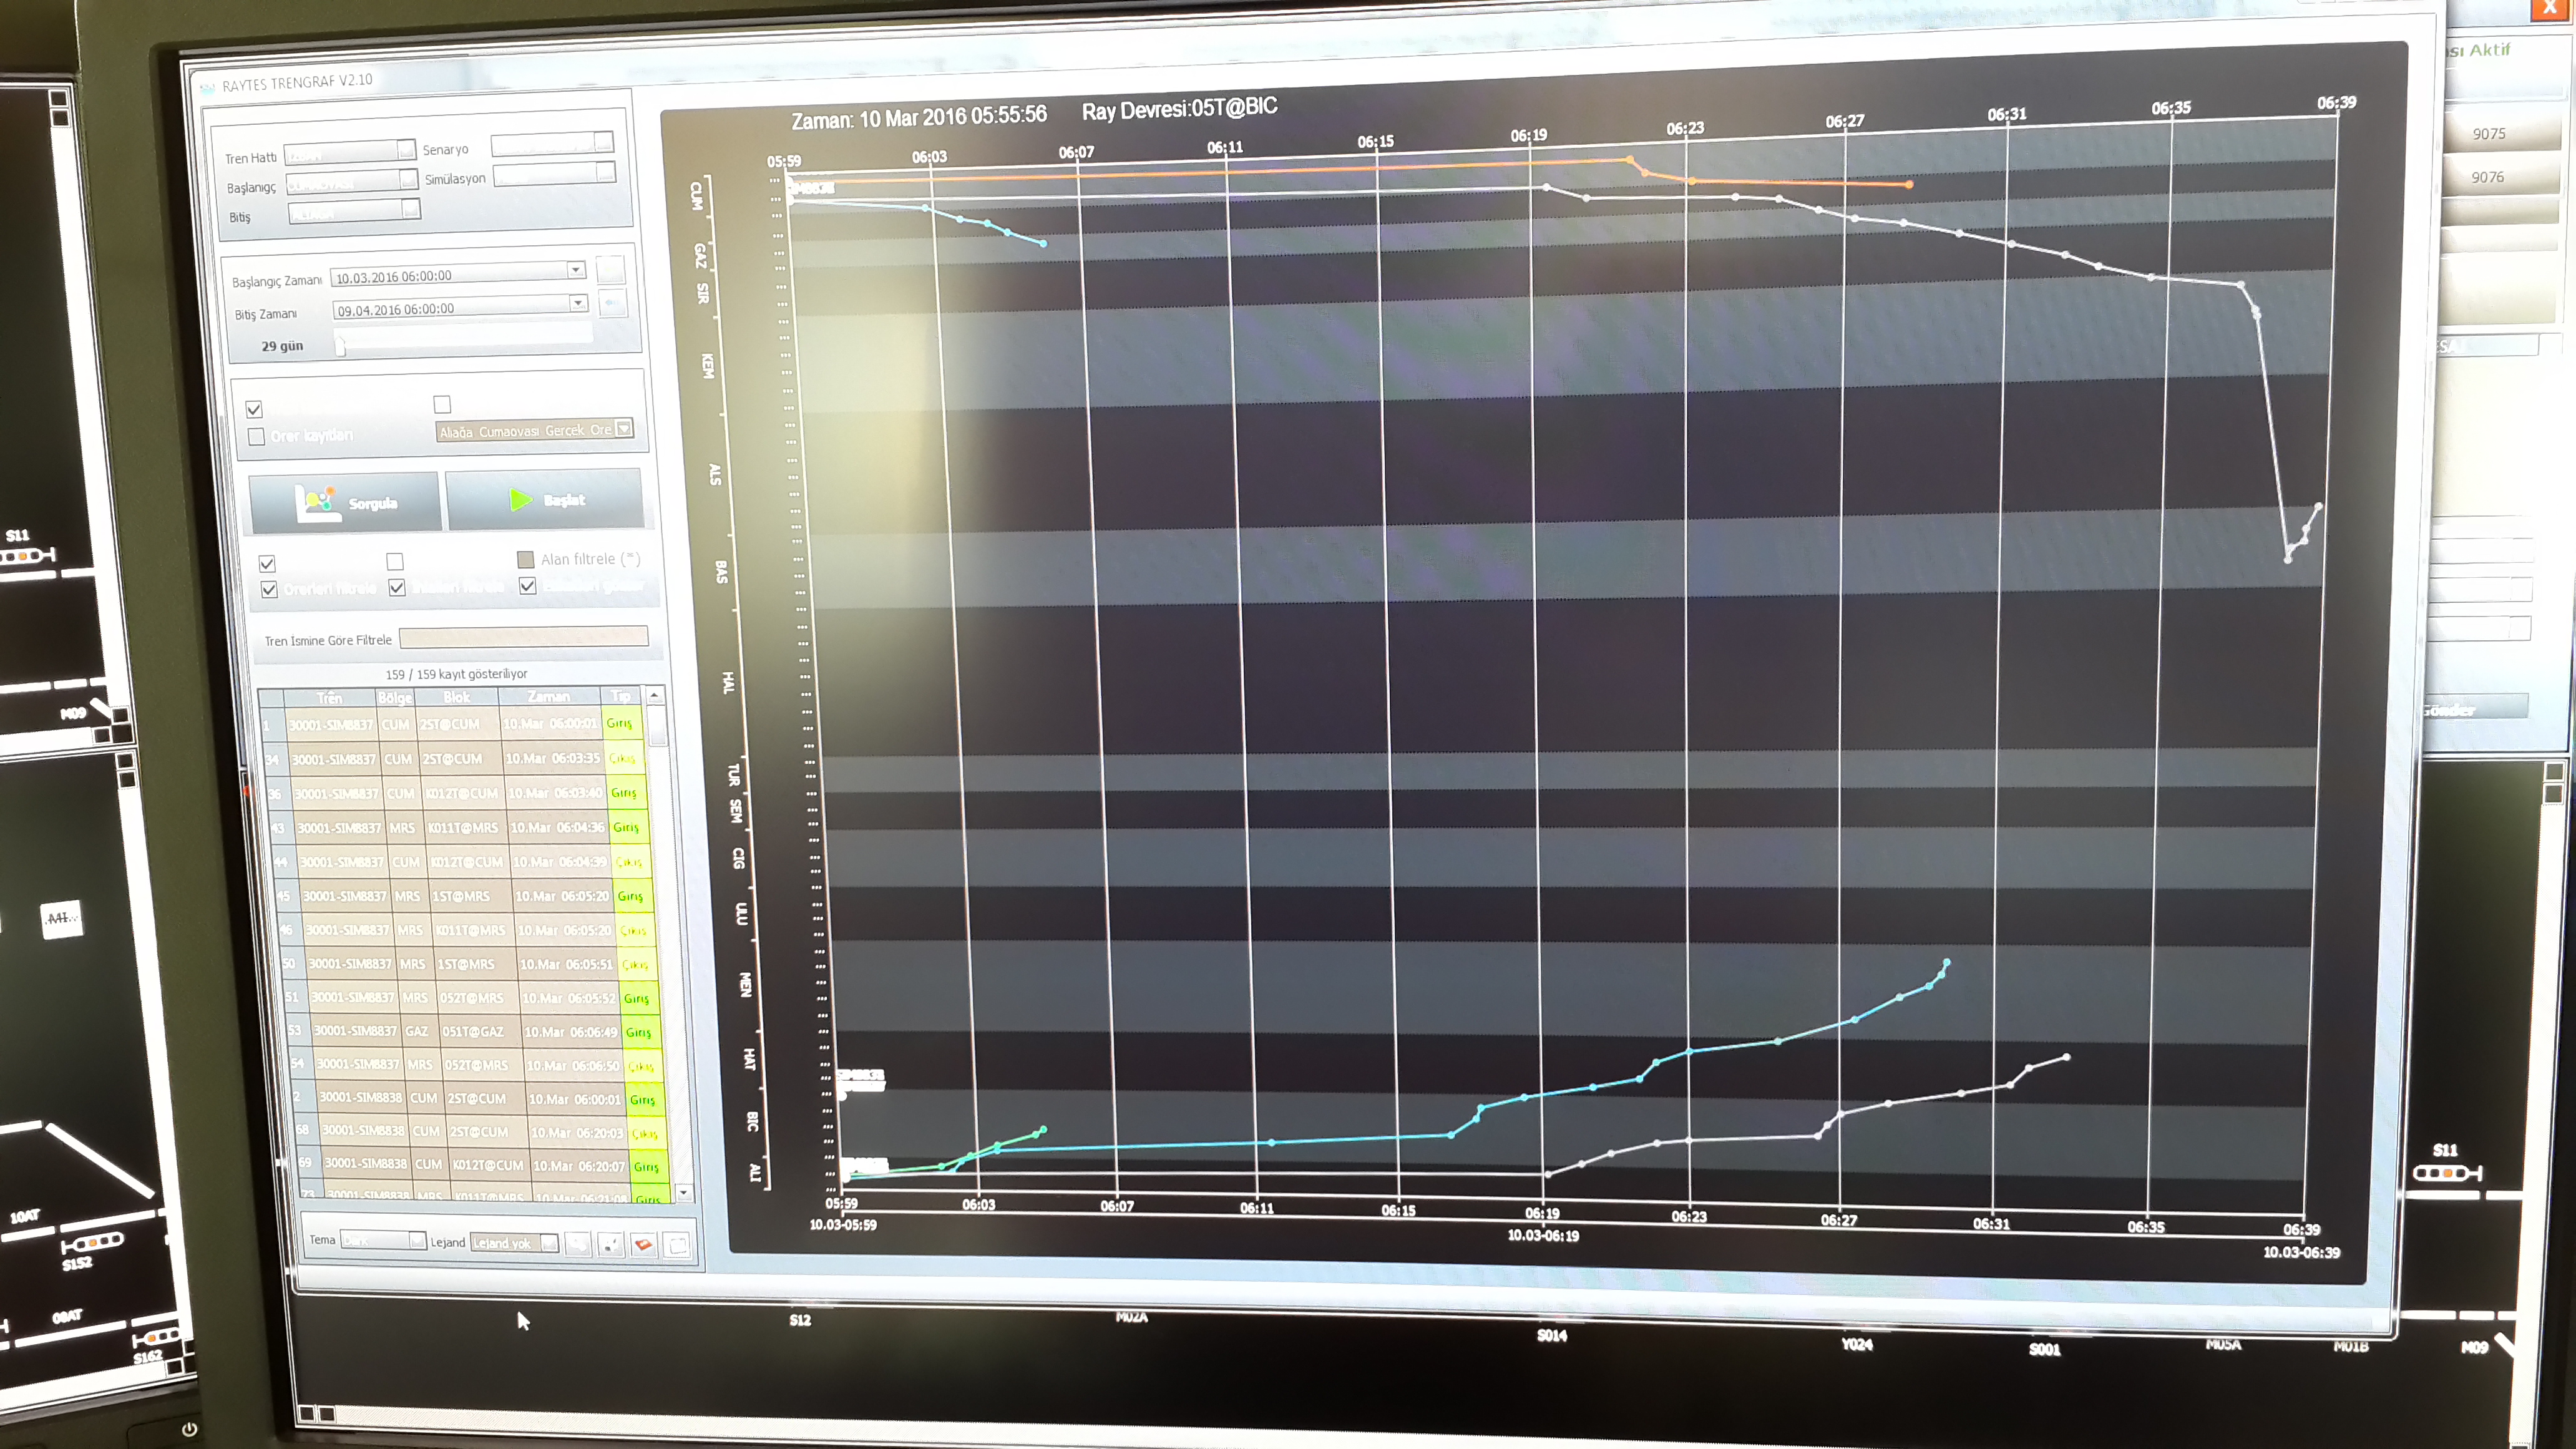
\includegraphics[width=8cm]{trenGrapSonuc.jpg}
  \caption{View of Train Movements}\label{fig:trenGrapSonuc}
  
\end{figure}
\begin{figure}[h!]
  \centering
  % Requires \usepackage{graphicx}
  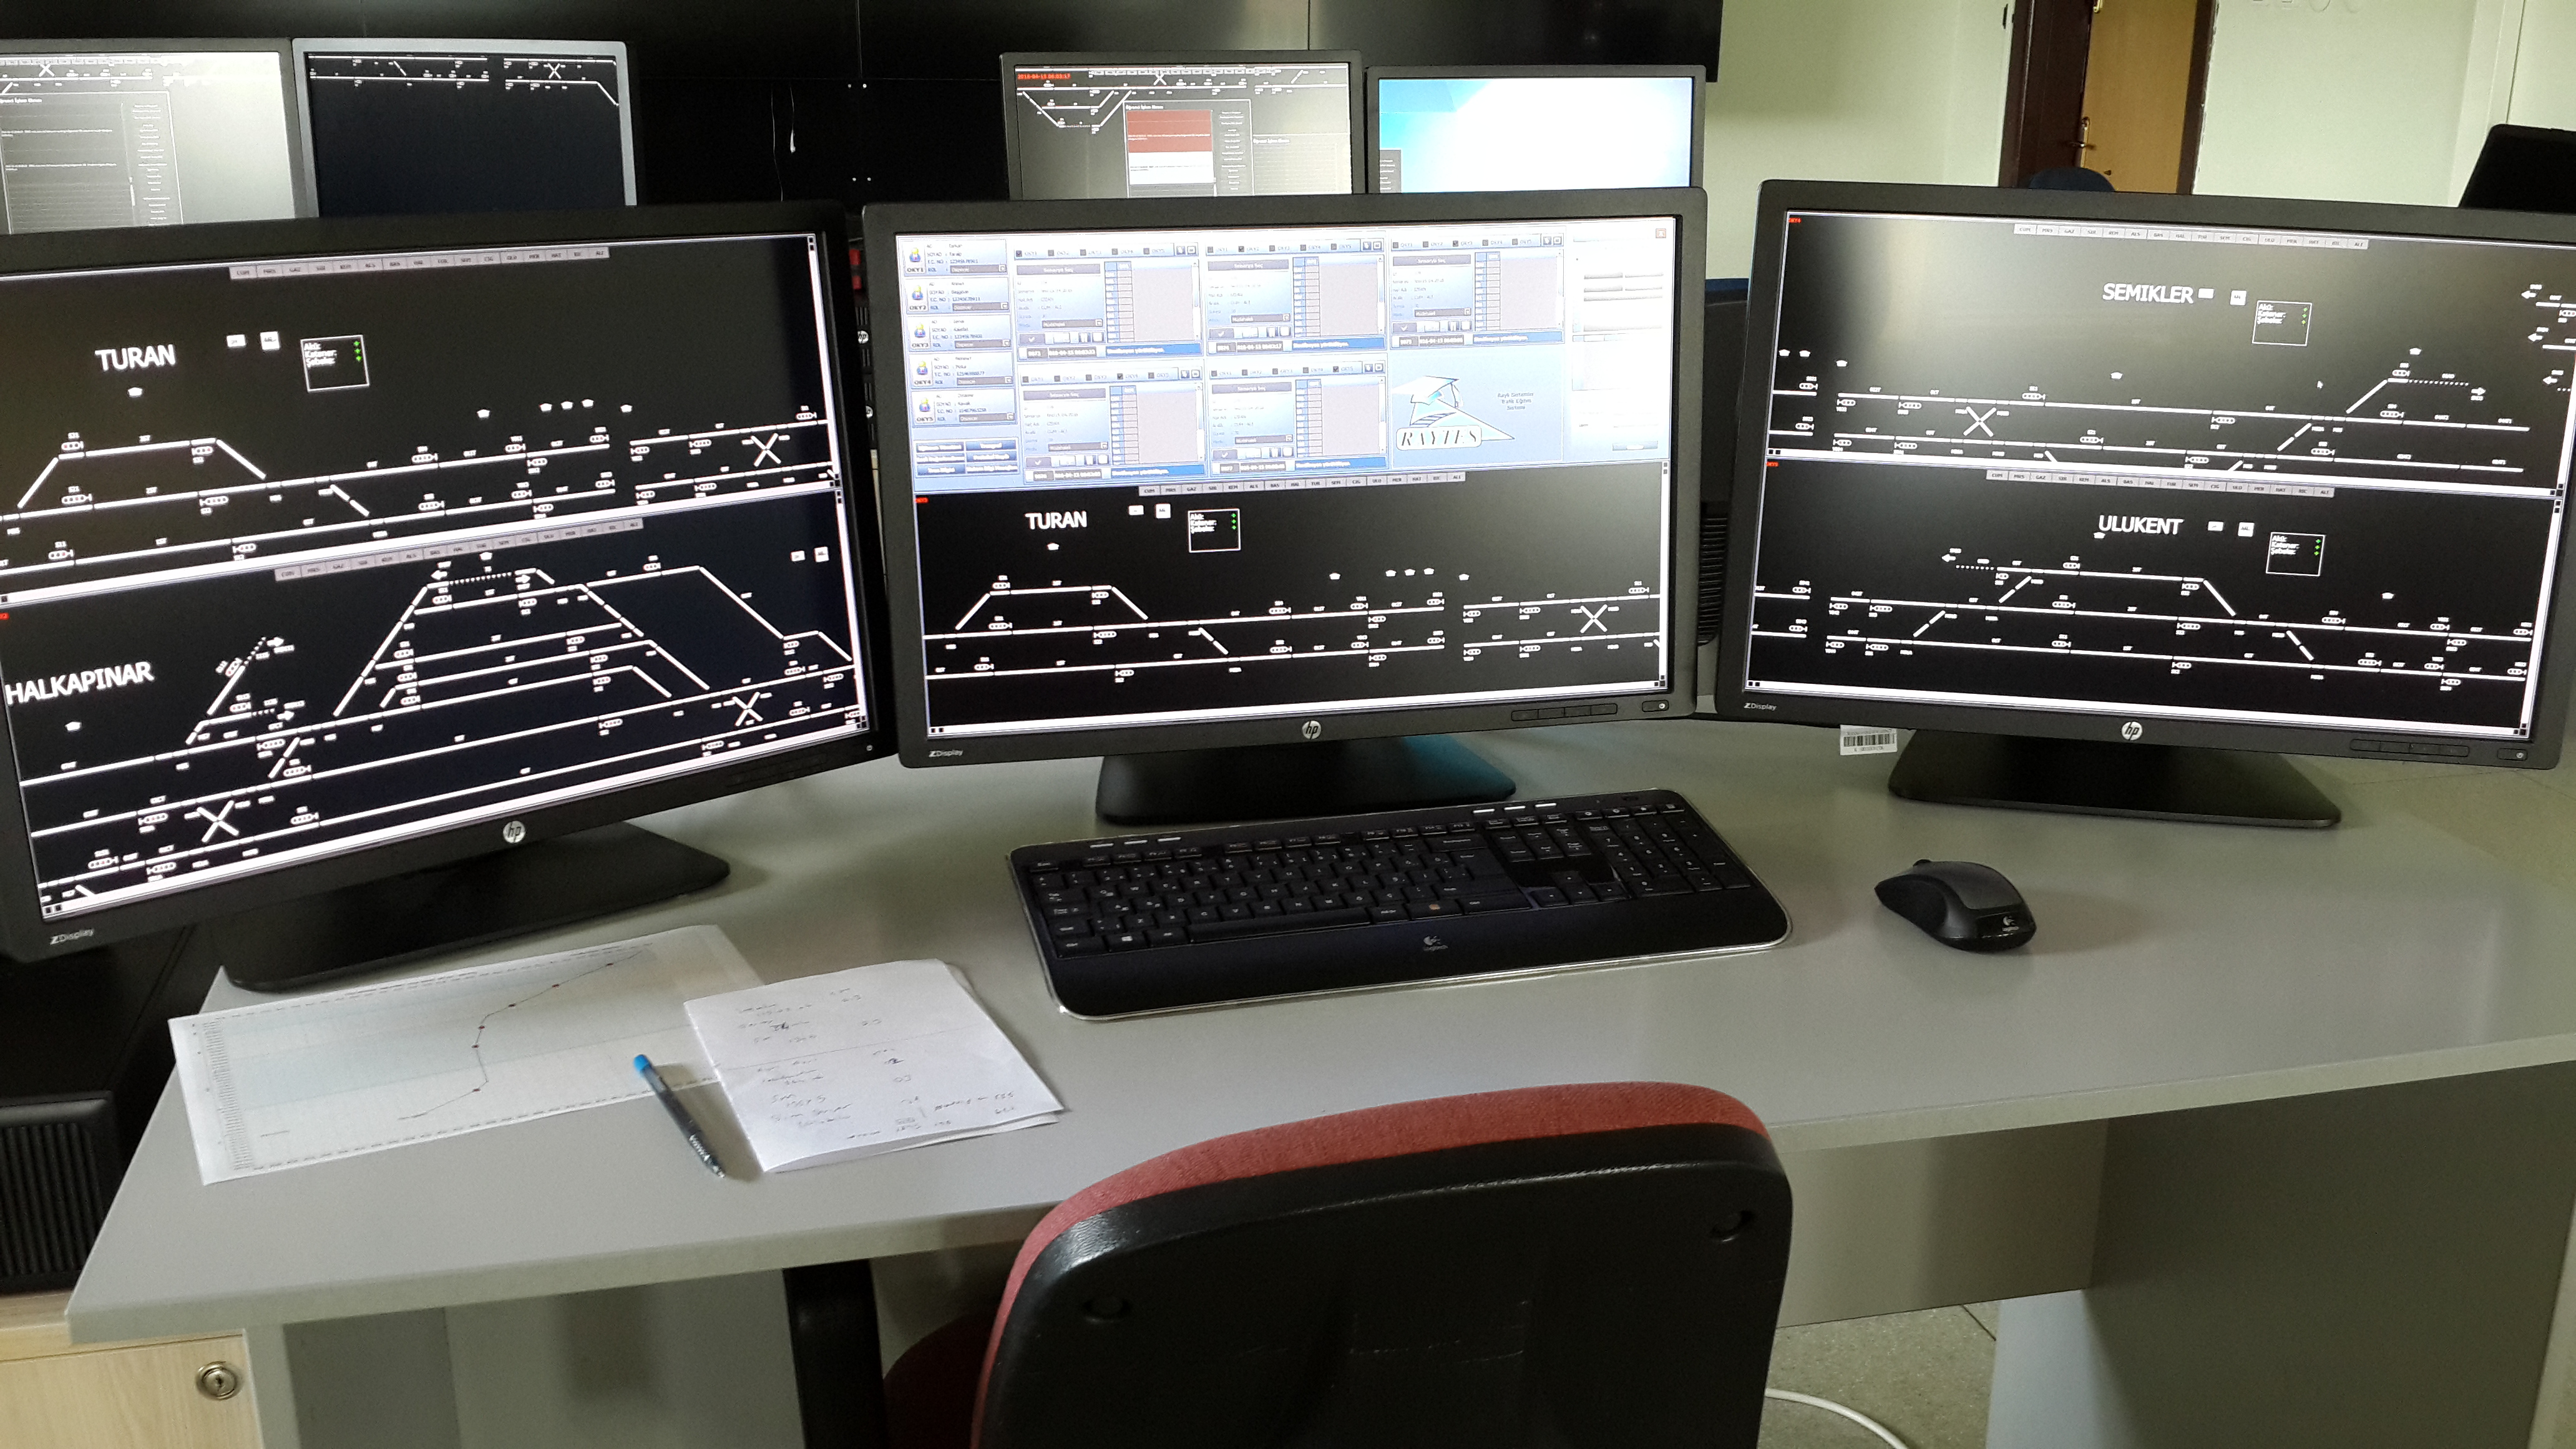
\includegraphics[width=8cm]{egitmenSonuc.jpg}
  \caption{The view of the training on the trainer console in 5 different simulations for 5 different students.}\label{fig:egitmenSonuc}
  
\end{figure}
\begin{figure}[h!]
  \centering
  % Requires \usepackage{graphicx}
  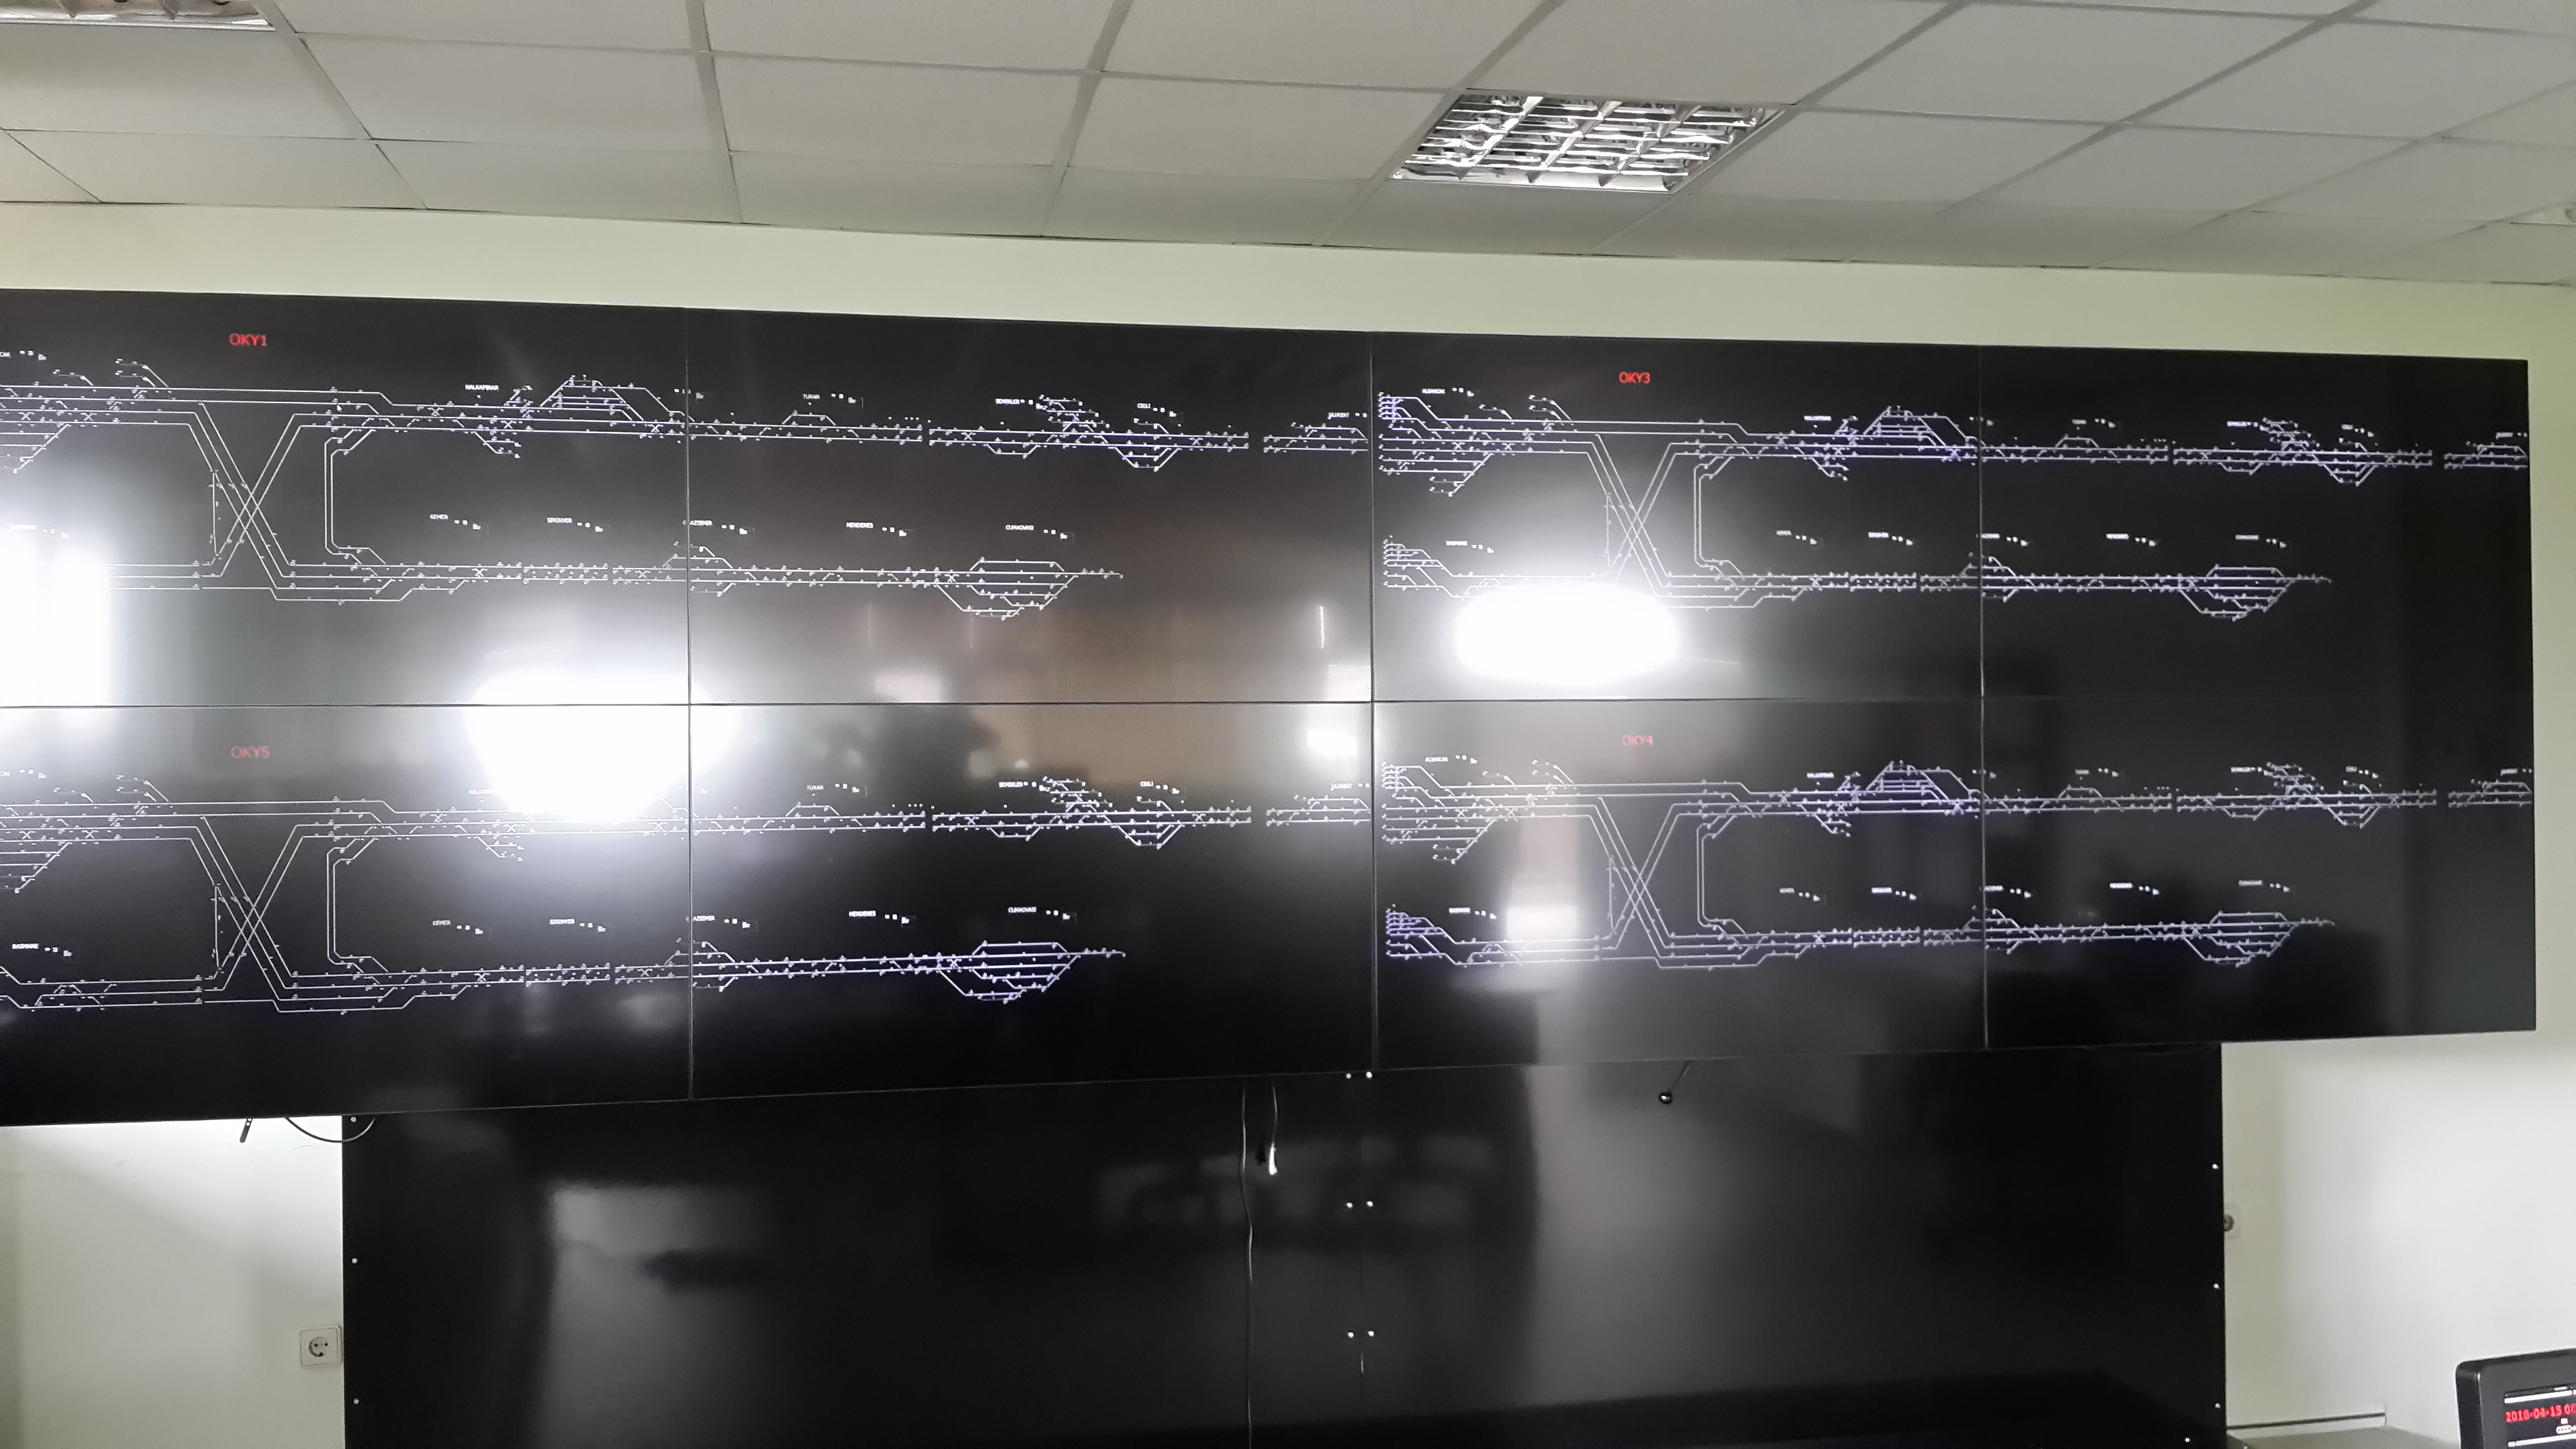
\includegraphics[width=8cm]{genisekranSonuc.jpg}
  \caption{The view of the screenshots of 4 different users on widescreen.}\label{fig:genisekranSonuc}
  
\end{figure}


\section{Conclusion}
Computer Simulations might be thought as a powerful tool for learning analysis, design and  interaction.
Fig.  13: The view of the screenshots of 4 different users on widescreen. 

Train traffic simulation has become an important tool in vital and critical level. Preventing the trains from collision and keeping them safe are among the most important aims of Train Control Systems.
	Providing train traffic control training for dispatchers in a distributed simulation system is the main purpose of this study. There are instructor console, 5 student consoles, a scenario-editor console and train graph tool in this system. Three actual train routes and 50 stations and interlocking areas in Turkey are used in the system. In this simulation system, the dispatchers might control the train traffic with various complexity levels. The success levels of the students in training outcomes might be measured with various tools. The instructor console makes decisions on the organization of the training and learning experiences and the classroom management, and provides response to individual students. The user is able to monitor and track the progression of 5 students via the simulation. In further studies, we will try to find the optimal solutions for train re-scheduling problems, and autonomous paths planned for trains. The dispatchers in such a case will only monitor the system.


% use section* for acknowledgment
\section*{Acknowledgment}


This study has been conducted with Rail Transit Systems Simulation Research Labs project (The Project Number 3920- S513000) for State Railways Administration of Turkey, which is part of the Rail Transit Systems research program, which has been funded by the National Research Institute of Electronics and Cryptology (TUBITAK BILGEM). We thank all project partners for their work and contributions in the project cycle.

\begin{thebibliography}{1}

\bibitem{FRISO}
A. D. Middelkoop and L. Loeve, “Simulation of traffic management with FRISO,” 2006, vol. 1, pp. 501–509.

\bibitem{ICVES}
M. Baohua, J. Wenzheng, C. Shaokuan, and L. Jianfeng, “A computer-aided multi-train simulator for rail traffic,” in IEEE International Conference on Vehicular Electronics and Safety, 2007. ICVES, 2007, pp. 1–5.

\bibitem{Sahin}
 I. Sahin, “Railway traffic control and train scheduling based oninter-train conflict management,” Transportation Research Part B: Methodological, vol. 33, no. 7, pp. 511–534, Sep. 1999.

\bibitem{network1}
V. Ginot, C. Le Page, and S. Souissi, “A multi-agents architecture to enhance end-user individual-based modelling,” Ecological modelling, vol. 157, no. 1, pp. 23–41, 2002.
\bibitem{network2}
D. Chen, S. J. Turner, W. Cai, and M. Xiong, “A decoupled federate architecture for high level architecture-based distributed simulation,” Journal of Parallel and Distributed Computing, vol. 68, no. 11, pp. 1487–1503, 2008.
\bibitem{network3}
A. Varga and others, “The OMNeT++ discrete event simulation system,” in Proceedings of the European simulation multiconference (ESM’2001), 2001, vol. 9, p. 65.
\bibitem{network4}
M. Pipattanasomporn, H. Feroze, and S. Rahman, “Multi-agent systems in a distributed smart grid: Design and implementation,” in Power Systems Conference and Exposition, 2009. PSCE’09. IEEE/PES, 2009, pp. 1–8.
 

\end{thebibliography}




% that's all folks
\end{document}


